\documentclass[11pt, oneside]{article}
\usepackage{geometry}
\geometry{letterpaper}
% packages
\usepackage{amsmath, amssymb}
\usepackage{cancel}
\usepackage{xcolor}
\usepackage{graphicx}


\title{ACT 2012\\Math Practice I}
\author{Daniel Topa}
%\date{}							% Activate to display a given date or no date

\begin{document}
\maketitle

%  %%  %%  %%  %%  %%  %%  %%  %%  %%  %%  %%  %%  %%  %%  %%  %%  %%  %%  %%  %%
\section{True/False}
\includegraphics[ width = 3in ]{images/"ACT 2012 I 01"}
\subsection{A. False}
Counterexample: a real number which is irrational: $\sqrt{2}$
\subsection{B. True}
Every integer $n$ is the rational number $\frac{n}{1}$
\subsection{C. False}
Counterexample: an integer which in not a whole number: $-1$.
\subsection{D. False}
The number $0$ is non-negative yet not positive.
\subsection{E. False}
The number $\pi$ is irrational. But the problem poses a finite approximation of $\pi$ which is rational: 
$$3.1416=\frac{31416}{10000}$$

%  %%  %%  %%  %%  %%  %%  %%  %%  %%  %%  %%  %%  %%  %%  %%  %%  %%  %%  %%  %%
\section{Rational numbers}
\includegraphics[ width = 3in ]{images/"ACT 2012 I 02"}
\subsection{F. Rational}
$$-3 = \frac{-3}{1}$$
\subsection{G. Irrational}
There are no integers $p$ and $q$ such that $$-\sqrt{3} = \frac{p}{q}$$.
\subsection{H. Rational}
$$\sqrt{9} = 3 = \frac{3}{1}$$
\subsection{J. Rational}
The symbol \% is Latin shorthand for \emph{per centum}: $$17\% = \frac{17}{100}$$.
\subsection{K. Rational}
$$p=8, \ q=10$$
Caveat: stricter definitions require that $p$ and $q$ be in simplest form. In this case the rational number is $\frac{4}{1}$.

%  %%  %%  %%  %%  %%  %%  %%  %%  %%  %%  %%  %%  %%  %%  %%  %%  %%  %%  %%  %%
\section{Precendence}
\includegraphics[ width = 3in ]{images/"ACT 2012 I 03"}
\subsection{D. $-22$}
%
\begin{equation}
	\begin{split}
		2^{3}-3\left[5 - \left(4-3^{2}\right) \right] 
			&= 2^{3}-3\left[5 - \left(4-9\right) \right] \\
			&= 2^{3}-3\left[5 - \left(-5 \right) \right] \\
			&= 2^{3}-3\left[10 \right] \\
			&= 2^{3}-30 \\
			&= 8-30 \\
			&= -22 \\
	\end{split}
%\label{eq:}
\end{equation}
%

%  %%  %%  %%  %%  %%  %%  %%  %%  %%  %%  %%  %%  %%  %%  %%  %%  %%  %%  %%  %%
\section{Regions}
\includegraphics[ width = 6in ]{images/"ACT 2012 I 04"}\\
The region represents everything outside of the ball of radius $2$ centered at $x=-3$. This is the complement of the region $-5 \le x \le -1$.
\subsection{F.}

%  %%  %%  %%  %%  %%  %%  %%  %%  %%  %%  %%  %%  %%  %%  %%  %%  %%  %%  %%  %%
\section{Remainders}
\includegraphics[ width = 6in ]{images/"ACT 2012 I 05"}
\subsection{C. $9$ inches}
Convert to feet: 10 yards = 30 feet of fabric. Each unit needs 2 ft 3in $= 2\frac{1}{4}$ feet of fabric.\\ 

\noindent Estimate: $12 \times 2\frac{1}{4} = 24 + 3 = 27$ ft. We can make one more item, for a total of $27 + 2\frac{1}{4} = 29\frac{1}{4}$ ft. Leftover $30-29\frac{1}{4}=\frac{3}{4}$ ft $=9$ in.

%  %%  %%  %%  %%  %%  %%  %%  %%  %%  %%  %%  %%  %%  %%  %%  %%  %%  %%  %%  %%
\section{Domain}
\includegraphics[ width = 6in ]{images/"ACT 2012 I 06"}
\subsection{G. $\mathbb{R}\backslash\left\{-1\right\}$}
The function is not defined when the denominator is $0$. Reduce function to simplest form and qualify denominator. Factor denominator: 
$$x^2-x-2 = (x+1)(x-2)$$
Simplify input fynction:
$$\frac{x-2}{x^2-x-2} = \frac{\cancel{x-2}}{(x+1)\cancel{(x-2)}} = \frac{1}{x+1}.$$
Therefore, the input function is not defined when $x=-1$.

%  %%  %%  %%  %%  %%  %%  %%  %%  %%  %%  %%  %%  %%  %%  %%  %%  %%  %%  %%  %%
\section{Prime numbers}
Memorize the primes less than 100:
$$\{2,3,5,7,11,13,17,19,23,29,31,37,41,43,47,53,59,61,67,71,73,79,83,89,97\}$$
\includegraphics[ width = 6in ]{images/"ACT 2012 I 07"}
\subsection{A. All are prime}
\subsection{{\color{blue}{B.}} $2$ is not prime}
\subsection{C. All are prime}
\subsection{D. All are prime}
\subsection{{\color{blue}{E.}} $1$ is not prime, by formal definition.}

%  %%  %%  %%  %%  %%  %%  %%  %%  %%  %%  %%  %%  %%  %%  %%  %%  %%  %%  %%  %%
\section{Precedence}
\includegraphics[ width = 6in ]{images/"ACT 2012 I 08"}
\subsection{F. $-7$}
%
\begin{equation}
	\begin{split}
		x-y(x+y) 
			&= (-4) - (-3) \left( (-4) - (-3)\right) \\
			&= (-4) - (-3) \left( -4 + 3 \right) \\
			&= (-4) - (-3) \left( -1\right) \\
			&= (-4) - 3 \\
			&= -7 \\
	\end{split}
%\label{eq:}
\end{equation}
%

%  %%  %%  %%  %%  %%  %%  %%  %%  %%  %%  %%  %%  %%  %%  %%  %%  %%  %%  %%  %%
\section{Real numbers}
\includegraphics[ width = 6in ]{images/"ACT 2012 I 09"}
\subsection{A. Rational $\frac{143}{100}$}
\subsection{B. Integer $1$}
\subsection{{\color{blue}{C.}} Not defined - division by $0$}
\subsection{D. Irrational}
\subsection{E. Irrational}

%  %%  %%  %%  %%  %%  %%  %%  %%  %%  %%  %%  %%  %%  %%  %%  %%  %%  %%  %%  %%
\section{Geometry}
\includegraphics[ width = 6in ]{images/"ACT 2012 I 10"}
Notation unknown.

%  %%  %%  %%  %%  %%  %%  %%  %%  %%  %%  %%  %%  %%  %%  %%  %%  %%  %%  %%  %%
\section{Distance}
\includegraphics[ width = 6in ]{images/"ACT 2012 I 11"}
\subsection{B. $210 = 40x - 45(x-1)$}
Foundation: distance = velocity times time 
$$d=vt$$.

\noindent Ashley's distance from origin $d_{1} = v_{1} t = 40t$\\
\noindent Ricky's distance from origin $d_{2} = v_{2} (t-1)= 45(t-1)$ for $t>1$\\

\noindent Distance between Ashley and Ricky: $D = d_{1} - d{2}$. When does $D=-210$? When
$$-210 = 40t - 45(t-1)$$

\noindent $t = 33$ hours.

%  %%  %%  %%  %%  %%  %%  %%  %%  %%  %%  %%  %%  %%  %%  %%  %%  %%  %%  %%  %%
\section{Algebra}
\includegraphics[ width = 6in ]{images/"ACT 2012 I 12"}
\subsection{H. $\left\{2\right\}$}
%
\begin{equation}
	\begin{split}
		5(x-3)+4 &= 5-2(x+1) \\
		5x - 15 + 4&= 5-2x-2 \\
		5x - 11&= 3-2x \\
		7x &= 14 \\
		x&=2
	\end{split}
%\label{eq:}
\end{equation}
%
\subsection{Check}
If $x=2$, $x-3=-11$, and $x+1=3$. Therefore $5(x-3)+4 = -5 + 4 = -1$ and $5-2(x+1) = 5-2\cdot 3 = -1$.


%  %%  %%  %%  %%  %%  %%  %%  %%  %%  %%  %%  %%  %%  %%  %%  %%  %%  %%  %%  %%
\section{Geometry}
\includegraphics[ width = 6in ]{images/"ACT 2012 I 13"}
\subsection{D. $\sqrt{17}$}
%
\begin{equation}
	BD = \sqrt{BE^{2} + DE^{2}}
\label{eq:13}
\end{equation}
%
Given $DE =3$, we need to find $BE$. Use
%
\begin{equation}
	BE = \sqrt{ AB^{2} + AE^{2} } = \sqrt{ 2^{2} + 2^{2} } = \sqrt{8}
%\label{eq:}
\end{equation}
%
By \eqref{eq:13}, 
%
\begin{equation}
	BD = \sqrt{3^{2} + \sqrt{8}^{2}}  = \sqrt{9 + 8} = \sqrt{17}
%\label{eq:}
\end{equation}
%


%  %%  %%  %%  %%  %%  %%  %%  %%  %%  %%  %%  %%  %%  %%  %%  %%  %%  %%  %%  %%
\section{Number Line}
\includegraphics[ width = 6in ]{images/"ACT 2012 I 14"}
\subsection{F. $5-(-8)$}

%  %%  %%  %%  %%  %%  %%  %%  %%  %%  %%  %%  %%  %%  %%  %%  %%  %%  %%  %%  %%
\section{Geometry}
\includegraphics[ width = 6in ]{images/"ACT 2012 I 15"}
\subsection{D. $1125\% = \frac{1125}{100} = 11.25$}

%  %%  %%  %%  %%  %%  %%  %%  %%  %%  %%  %%  %%  %%  %%  %%  %%  %%  %%  %%  %%
\section{Factor quadratics}
\includegraphics[ width = 6in ]{images/"ACT 2012 I 16"}
\subsection{G. $6x^{2} + 6x -36 = 6(x^{2}+x-6) = 6(x-2)(x+3)$}

%  %%  %%  %%  %%  %%  %%  %%  %%  %%  %%  %%  %%  %%  %%  %%  %%  %%  %%  %%  %%
\section{Binomial Theorem}
\includegraphics[ width = 6in ]{images/"ACT 2012 I 17"}
\subsection{A. $4845$}

Number of unique combinations of $k=4$ distinct items from a pool of $n=20$ items is given by ``binomial n k'':
%
\begin{equation}
	\binom{n}{k} = \frac{n!} {k!(n-k)!}
%\label{eq:}
\end{equation}
%
For this problem
%
\begin{equation}
	\binom{n}{k} = \frac{20!} {4!(20-4)!} = \frac{20!} {4!16!} = \frac{20\cdot19\cdot18\cdot17\cdot\cancel{16!}} {4!\cancel{16!}}
%\label{eq:}
\end{equation}
%
Further simplification
%
\begin{equation}
	\frac{20\cdot19\cdot18\cdot17} {4!} = 5\cdot 19 \cdot 3 \cdot 17 = 4845
%\label{eq:}
\end{equation}
%

%  %%  %%  %%  %%  %%  %%  %%  %%  %%  %%  %%  %%  %%  %%  %%  %%  %%  %%  %%  %%
\section{Shapes}
\includegraphics[ width = 6in ]{images/"ACT 2012 I 18"}
\subsection{K. parallelogram}

%  %%  %%  %%  %%  %%  %%  %%  %%  %%  %%  %%  %%  %%  %%  %%  %%  %%  %%  %%  %%
\section{Algebra}
\includegraphics[ width = 6in ]{images/"ACT 2012 I 19"}
\subsection{A. $17x +12$}
%
\begin{equation}
	\begin{split}
		2x-3\left[x-2(3x-2) \right] 
			&= 2x-3\left[ x-6x+4 \right] \\
			&= 2x-3x +18x +12  \\
			&= 2x-3x +18x +12  \\
			&= 17x +12  \\
	\end{split}
%\label{eq:}
\end{equation}
%

%  %%  %%  %%  %%  %%  %%  %%  %%  %%  %%  %%  %%  %%  %%  %%  %%  %%  %%  %%  %%
\section{Exponents}
\includegraphics[ width = 6in ]{images/"ACT 2012 I 20"}
\subsection{H. $\frac{1}{16}$}
%
\begin{equation}
	-4^{-2} = \frac{1}{-4^{2}} = \frac{1}{(-4)(-4)} = \frac{1}{16}
%\label{eq:}
\end{equation}
%


%  %%  %%  %%  %%  %%  %%  %%  %%  %%  %%  %%  %%  %%  %%  %%  %%  %%  %%  %%  %%
\section{Complex numbers}
\includegraphics[ width = 6in ]{images/"ACT 2012 I 21"}
\subsection{B. $10+2i$}

Product of complex numbers:
$$(x_{1} + i y_{1}) (x_{2} + i y_{2}) = x_{1}x_{2} + y_{1}y_{2} + i (x_{1}y_{2} + x_{2}y_{1})$$

%
\begin{equation}
	(-1+i3)(2+i4) = -2 - (i^{2}) 12 + i (-4+6) = -2 +12 + i 2 = 10 + i2
%\label{eq:}
\end{equation}
%

%  %%  %%  %%  %%  %%  %%  %%  %%  %%  %%  %%  %%  %%  %%  %%  %%  %%  %%  %%  %%
\section{Geometry}
\includegraphics[ width = 6in ]{images/"ACT 2012 I 22"}
\subsection{K. $\frac{1}{2}(105 + 4\pi) = 52\frac{1}{2} + 2\pi$}

Use the partition
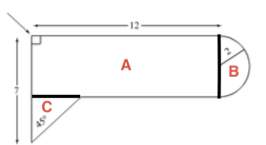
\includegraphics[ width = 2in ]{images/partition}

Area $A$:
$$A = 12 \times 4 = 48$$

Area $B$:
$$B = \frac{1}{2} \pi r^{2} = \frac{1}{2} \pi 4 = 2\pi$$

Area $C$:
$$C = \frac{1}{2}3\times 3= 4\frac{1}{2}$$

Total area:
$$A+B+C = 52\frac{1}{2} + 2\pi$$

%  %%  %%  %%  %%  %%  %%  %%  %%  %%  %%  %%  %%  %%  %%  %%  %%  %%  %%  %%  %%
\section{Factoring}
\includegraphics[ width = 6in ]{images/"ACT 2012 I 23"}
\subsection{C. $\frac{12\sqrt{10}}{\sqrt{3}}$}
%
\begin{equation}
	\frac{12\sqrt{20}}{\sqrt{6}} = 12 \sqrt{\frac{20}{6}} = 12 \sqrt{\frac{10}{3}} = \frac{12\sqrt{10}}{\sqrt{3}}
%\label{eq:}
\end{equation}
%

%  %%  %%  %%  %%  %%  %%  %%  %%  %%  %%  %%  %%  %%  %%  %%  %%  %%  %%  %%  %%
\section{Symmetry}
\includegraphics[ width = 6in ]{images/"ACT 2012 I 24"}
\subsection{F. Symmetry with respect to the $x-$axis}

%  %%  %%  %%  %%  %%  %%  %%  %%  %%  %%  %%  %%  %%  %%  %%  %%  %%  %%  %%  %%
\section{Geometry}
\includegraphics[ width = 6in ]{images/"ACT 2012 I 25"}
%\subsection{F. Symmetry with respect to the $x-$axis}

%  %%  %%  %%  %%  %%  %%  %%  %%  %%  %%  %%  %%  %%  %%  %%  %%  %%  %%  %%  %%
\section{Symmetry}
\includegraphics[ width = 6in ]{images/"ACT 2012 I 26"}
\subsection{G. $\frac{2}{5}$}

$$\left\{ 1, 2^{\star}, 3^{\star}, 4, 5^{\star}, 6, 7^{\star}, 8, 9, 10, 11^{\star}, 12, 13^{\star}, 14, 15, 16, 17^{\star}, 18, 19^{\star}, 20 \right\}$$

Of the $20$ numbers, $8$ are prime. As a fraction, $\frac{8}{20} = \frac{2}{5}$ are prime.

%  %%  %%  %%  %%  %%  %%  %%  %%  %%  %%  %%  %%  %%  %%  %%  %%  %%  %%  %%  %%
\section{Powers}
\includegraphics[ width = 6in ]{images/"ACT 2012 I 27"}
\subsection{C. $288a\sqrt{10b^{3}}$}

$$\left(6\sqrt{48a}\right)\left(4\sqrt{30ab^{3}}\right) = 24 \sqrt{1440a^{2}b^{3}} = 24\cdot 12 a \sqrt{10b^{3}} = 288a\sqrt{10b^{3}}$$

%  %%  %%  %%  %%  %%  %%  %%  %%  %%  %%  %%  %%  %%  %%  %%  %%  %%  %%  %%  %%
\section{Algebra}
\includegraphics[ width = 6in ]{images/"ACT 2012 I 28"}
\subsection{K. $-1$}

$$\frac{a-b}{b-a} = \frac{\cancel{a-b}}{(-1)\cancel{(a-b)}} = -1$$


%  %%  %%  %%  %%  %%  %%  %%  %%  %%  %%  %%  %%  %%  %%  %%  %%  %%  %%  %%  %%
\section{Logarithms}
\includegraphics[ width = 6in ]{images/"ACT 2012 I 29"}
\subsection{A. $a+b+\frac{1}{2}(1+a)$}

$$\log_{2}{35\sqrt{6}} 
	= \log_{2} \left( 5 \cdot 7 \cdot 6^{\frac{1}{2}}\right) 
	= \log_{2} \left( 5 \cdot 7 \cdot 2^{\frac{1}{2}}3^{\frac{1}{2}}\right) 
	= a + b + \frac{1}{2}\left( 1+a\right)$$

%  %%  %%  %%  %%  %%  %%  %%  %%  %%  %%  %%  %%  %%  %%  %%  %%  %%  %%  %%  %%
\section{Geometry}
\includegraphics[ width = 6in ]{images/"ACT 2012 I 30"}
\subsection{H. $\angle ECB$}

\end{document}